\section{Resultater}
Ved testing av en enkelt halvadder fikk vi følgende resultater:

\begin{table}[!htb]
    \centering
    \caption{Halvadder resultater}
    \begin{tabular}{|c|c|c|c|c|c|}
        \hline
        \multicolumn{4}{|c|}{\textbf{Verdier fra forarbeid}} & \multicolumn{2}{c|}{\textbf{Målte verdier}} \\ \hline
        \textbf{A}    & \textbf{B} & \textbf{Sum}  & \textbf{Carry}  & \textbf{Sum}  & \textbf{Carry}\\ \hline
        0             & 0 & 0 & 0 &  0  & 0 \\ \hline
        0             & 1 & 1 & 0 &  1  & 0 \\ \hline
        1             & 0 & 1 & 0 &  1  & 0 \\ \hline
        1             & 1 & 0 & 1 &  0  & 1 \\ \hline
    \end{tabular}
\end{table}

Ved testing av ferdigkoblet absoluttverdikrets fikk vi følgende resultater:

\begin{table}[!htb]
  \caption{Absoluttverdikrets resultater}
  \begin{tabular}{c c c c c|c c}
    \multicolumn{5}{c|}{\textbf{Verdier fra forarbeid}} & \multicolumn{2}{c}{\textbf{Målte verdier}} \\ \hline
    \textbf{Binary} & \textbf{Hex} & \textbf{Decimal}  & \textbf{Binary(Abs)}  & \textbf{Hex(Abs)}  & \textbf{Binary(Input)} &  \textbf{Hex(Output)}\\ \hline
    0111  & 0x7 & 7 & 0111  & 0x7 & 0111  & 0x7 \\
    0110  & 0x6 & 6 & 0110  & 0x6 & 0110  & 0x6 \\
    0101  & 0x5 & 5 & 0101  & 0x5 & 0101  & 0x5 \\
    0100  & 0x4 & 4 & 0100  & 0x4 & 0100  & 0x4 \\
    0011  & 0x3 & 3 & 0011  & 0x3 & 0011  & 0x3 \\
    0010  & 0x2 & 2 & 0010  & 0x2 & 0010  & 0x2 \\
    0001  & 0x1 & 1 & 0001  & 0x1 & 0001  & 0x1 \\
    0000  & 0x0 & 0 & 0000  & 0x0 & 0000  & 0x0 \\ \hline
    1111  & 0xF & -1 & 1111  & 0x1 & 1111  & 0x1 \\
    1110  & 0xE & -2 & 1110  & 0x2 & 1110  & 0x2 \\
    1101  & 0xD & -3 & 1101  & 0x3 & 1101  & 0x3 \\
    1100  & 0xC & -4 & 1100  & 0x4 & 1100  & 0x4 \\
    1011  & 0xB & -5 & 1011  & 0x5 & 1011  & 0x5 \\
    1010  & 0xA & -6 & 1010  & 0x6 & 1010  & 0x6 \\
    1001  & 0x9 & -7 & 1001  & 0x7 & 1001  & 0x7 \\
    1000  & 0x8 & -8 & 1000  & 0x8 & 1000  & 0x8 \\

  \end{tabular}
  \label{Tabell:5}
\end{table}

\clearpage

Ved testing av forplantningstid fikk vi følgende resultater:

\begin{figure}
  \centering
  \caption{Tidsforsinkelse for kritisk sti}
  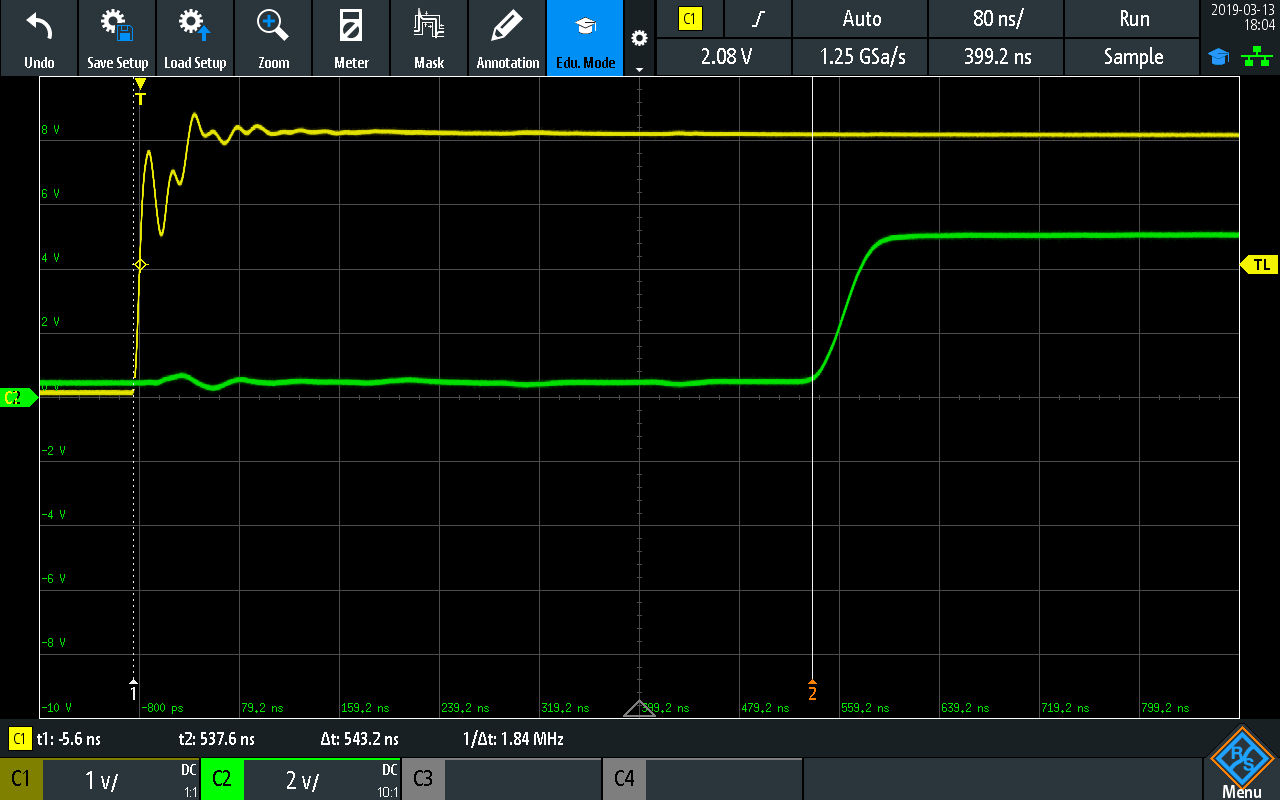
\includegraphics[width=14cm]{Bilder/fosinkelse.png}
\end{figure}

\begin{table}[!htb]
  \centering
  \caption{Tidsforsinkelse for kritisk sti}
  \begin{tabular}{c c c|c c c}
    \multicolumn{3}{c|}{\textbf{Tidsforsinkelse}} & \multicolumn{3}{c}{\textbf{Maksimal klokkefrekvens}} \\ \hline
    \textbf{Utregnet} & \textbf{Målt} & \textbf{Avvik} & \textbf{Utregnet} & \textbf{Målt} & \textbf{Avvik} \\ \hline
    655 ns & 543 ns & 112 ns & 1.53 MHz & 1.84 MHz & 0.31 MHz\\
  \end{tabular}
\end{table}

Ved testing av falltid og stigetid over kritisk sti fikk vi følgende resultater:

\begin{figure}
  \centering
  \caption{Falltid XOR}
  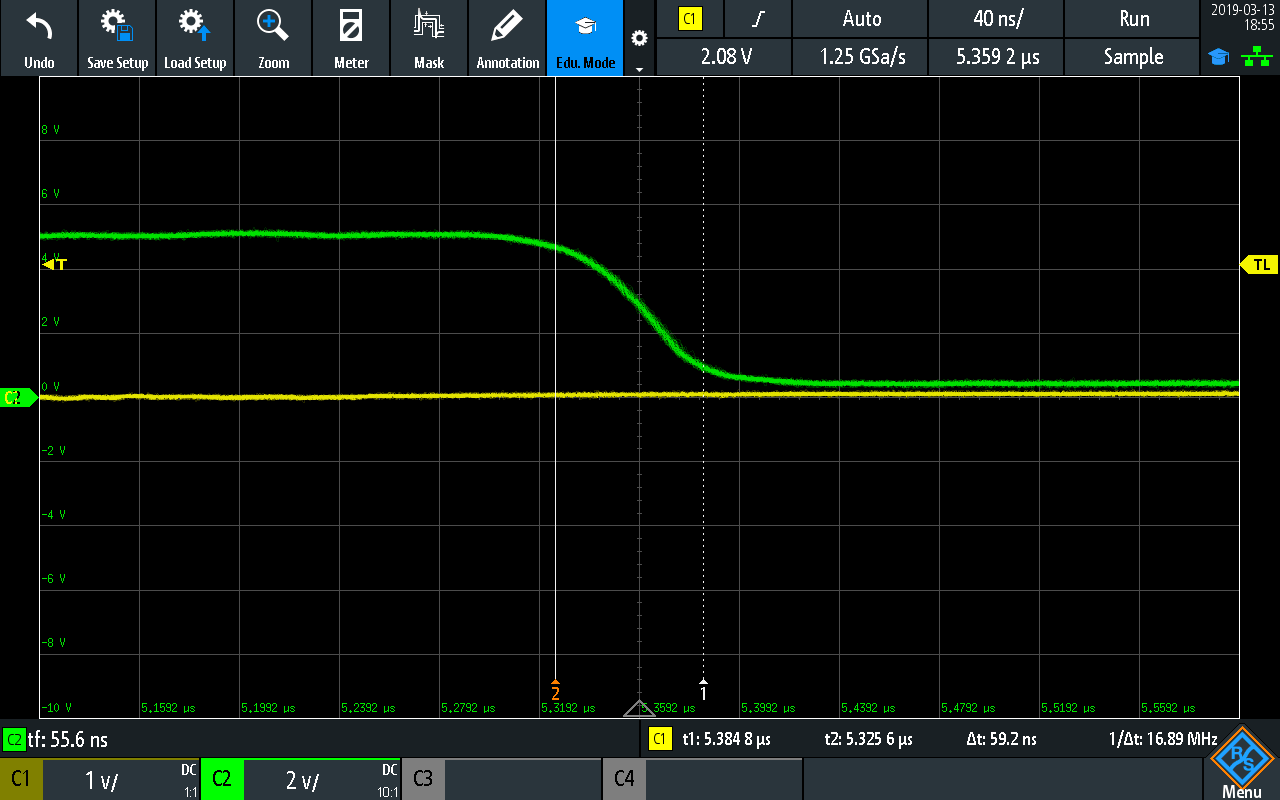
\includegraphics[width=14cm]{Bilder/Fall.png}
\end{figure}

\begin{figure}
  \centering
  \caption{Stigetid XOR}
  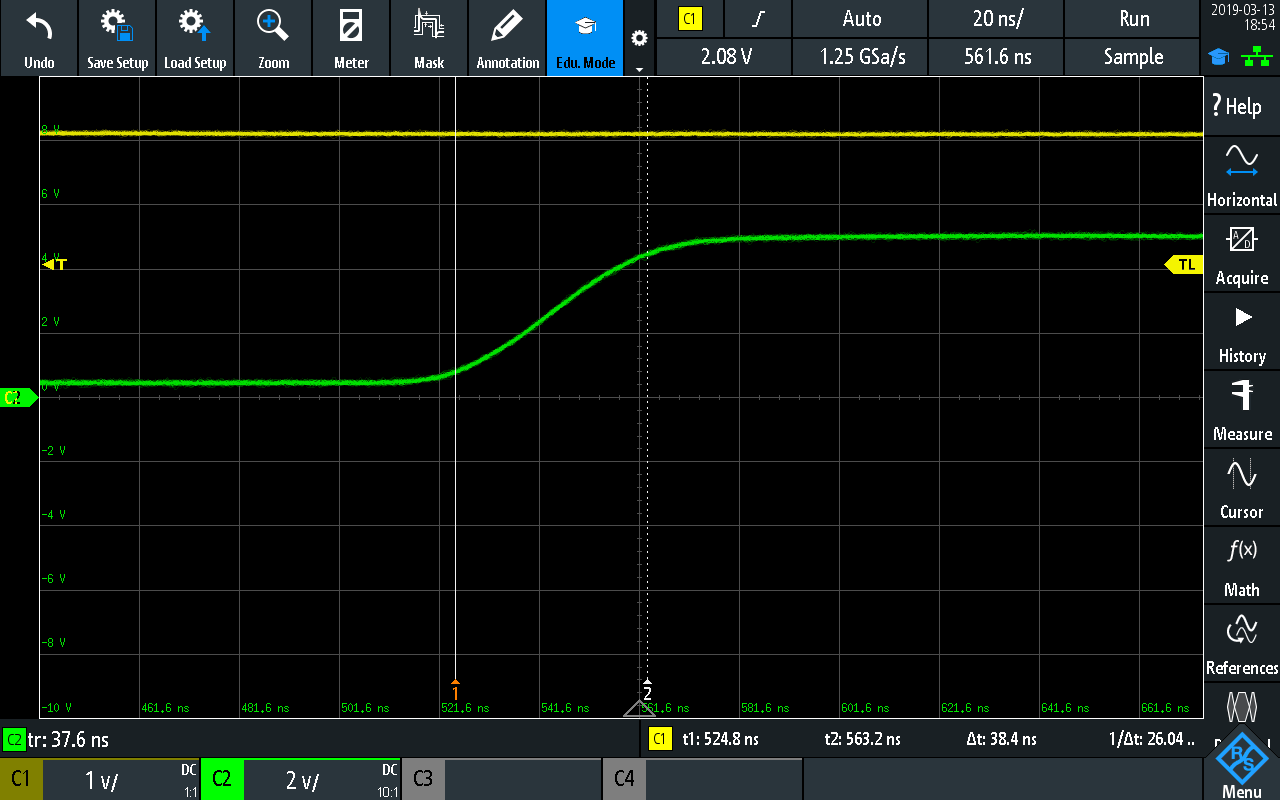
\includegraphics[width=14cm]{Bilder/Rise.png}
\end{figure}

\begin{figure}
  \centering
  \caption{Falltid AND}
  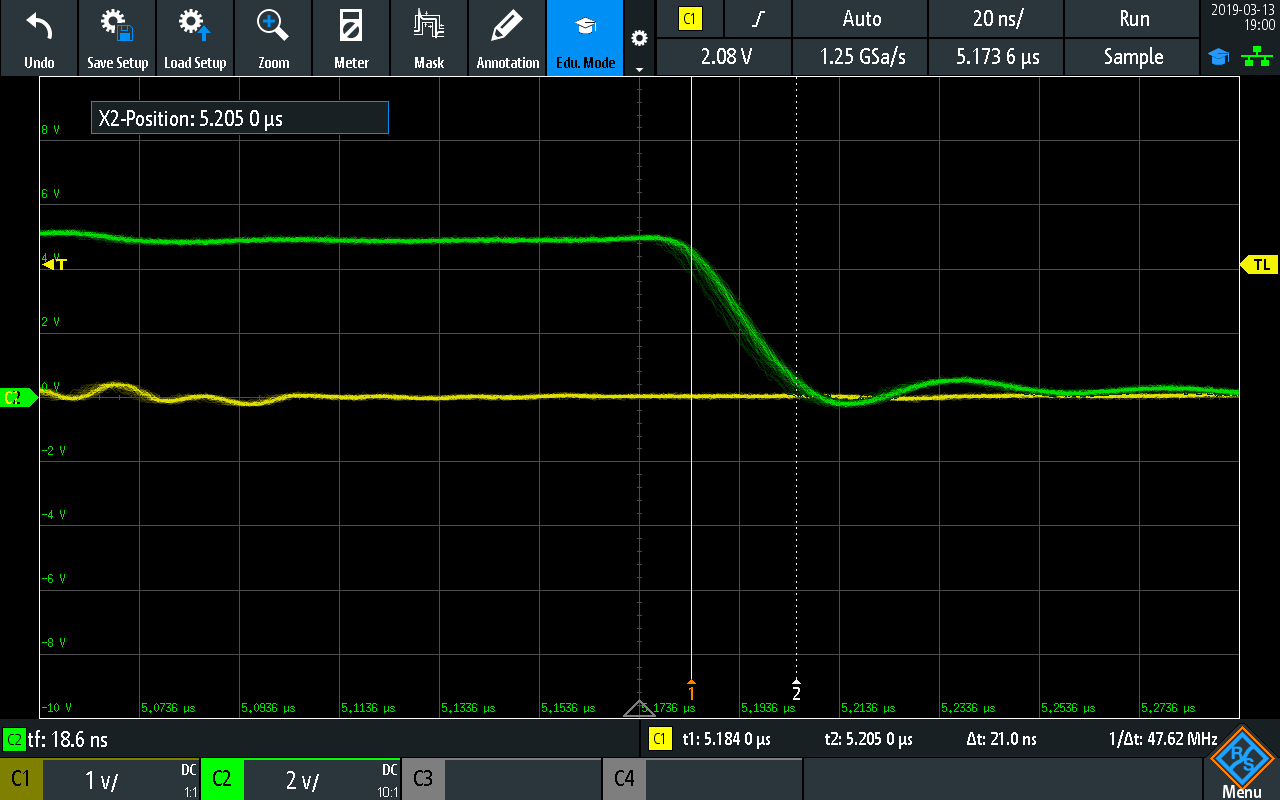
\includegraphics[width=14cm]{Bilder/Fall_and.png}
\end{figure}

\begin{figure}
  \centering
  \caption{Stigetid AND}
  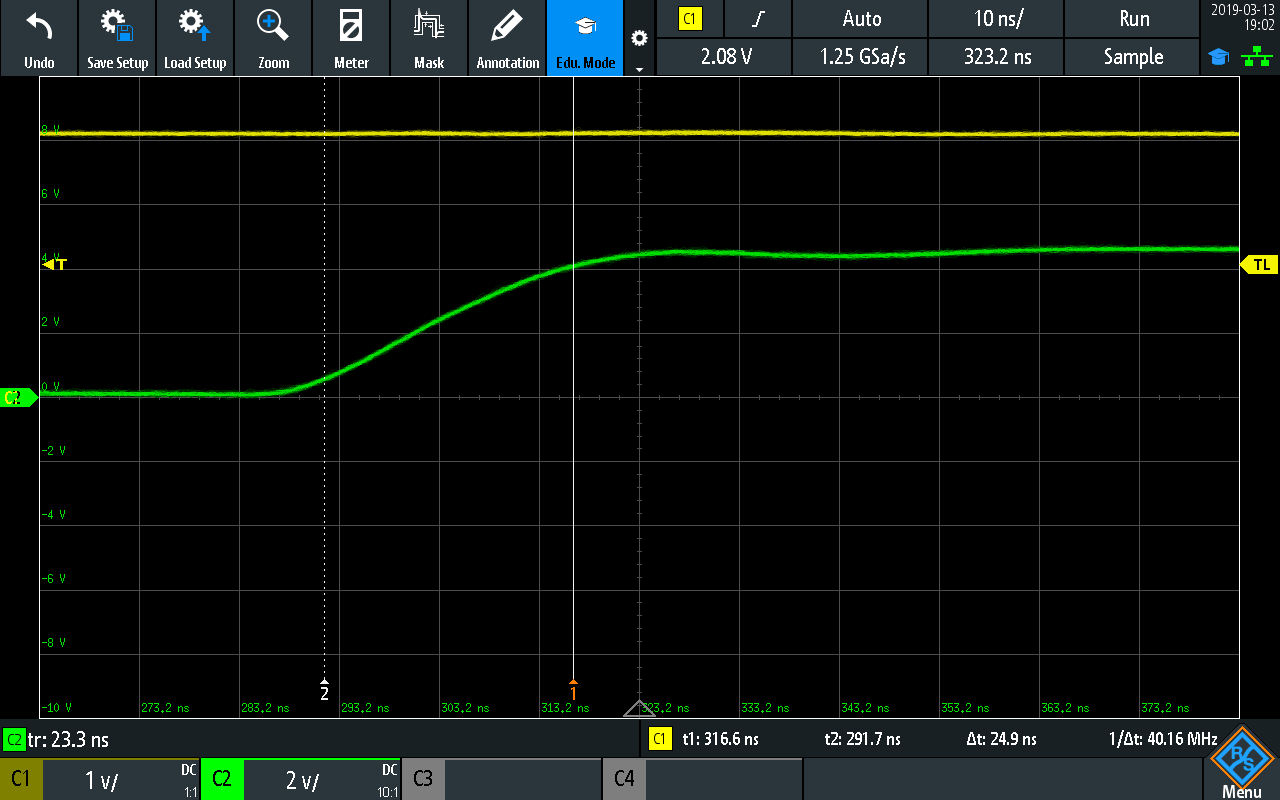
\includegraphics[width=14cm]{Bilder/Rise_and.png}
\end{figure}


\begin{table}
  \centering
  \caption{Stigetider og falltider}
  \begin{tabular}{c|c c}
     & \textbf{Stigetid} & \textbf{Falltid} \\ \hline
     \textbf{XOR} & 37.6 ns & 55.6 ns \\
     \textbf{AND} & 23.3 ns & 18.6 ns \\

  \end{tabular}
  \label{stigetidstuff}
\end{table}
